\documentclass{beamer}

%
% Choose how your presentation looks.
%
% For more themes, color themes and font themes, see:
% http://deic.uab.es/~iblanes/beamer_gallery/index_by_theme.html
%
\mode<presentation>
{
  \usetheme{default}      % or try Darmstadt, Madrid, Warsaw, ...
  \usecolortheme{default} % or try albatross, beaver, crane, ...
  \usefonttheme{default}  % or try serif, structurebold, ...
  \setbeamertemplate{navigation symbols}{}
  \setbeamertemplate{caption}[numbered]
  \setbeamertemplate{footline}[page number]
  \setbeamercolor{frametitle}{fg=white}
  \setbeamercolor{footline}{fg=black}
} 

\usepackage[english]{babel}
\usepackage[utf8x]{inputenc}
\usepackage{tikz}
\usepackage{listings}
\usepackage{courier}

\xdefinecolor{darkblue}{rgb}{0.1,0.1,0.7}
\xdefinecolor{dianablue}{rgb}{0.18,0.24,0.31}
\definecolor{commentgreen}{rgb}{0,0.6,0}
\definecolor{stringmauve}{rgb}{0.58,0,0.82}

\lstset{ %
  backgroundcolor=\color{white},      % choose the background color
  basicstyle=\ttfamily\small,         % size of fonts used for the code
  breaklines=true,                    % automatic line breaking only at whitespace
  captionpos=b,                       % sets the caption-position to bottom
  commentstyle=\color{commentgreen},  % comment style
  escapeinside={\%*}{*)},             % if you want to add LaTeX within your code
  keywordstyle=\color{blue},          % keyword style
  stringstyle=\color{stringmauve},    % string literal style
  showstringspaces=false,
  showlines=true
}

\lstdefinelanguage{scala}{
  morekeywords={abstract,case,catch,class,def,%
    do,else,extends,false,final,finally,%
    for,if,implicit,import,match,mixin,%
    new,null,object,override,package,%
    private,protected,requires,return,sealed,%
    super,this,throw,trait,true,try,%
    type,val,var,while,with,yield},
  otherkeywords={=>,<-,<\%,<:,>:,\#,@},
  sensitive=true,
  morecomment=[l]{//},
  morecomment=[n]{/*}{*/},
  morestring=[b]",
  morestring=[b]',
  morestring=[b]"""
}

\title[2016-11-07-diana-file-formats]{File formats for physics data}
\author{Jim Pivarski}
\institute{Princeton -- DIANA}
\date{November 7, 2016}

\begin{document}

\logo{\pgfputat{\pgfxy(0.11, 8)}{\pgfbox[right,base]{\tikz{\filldraw[fill=dianablue, draw=none] (0 cm, 0 cm) rectangle (50 cm, 1 cm);}}}\pgfputat{\pgfxy(0.11, -0.6)}{\pgfbox[right,base]{\tikz{\filldraw[fill=dianablue, draw=none] (0 cm, 0 cm) rectangle (50 cm, 1 cm);}
\includegraphics[height=0.99 cm]{diana-hep-logo.png}\tikz{\filldraw[fill=dianablue, draw=none] (0 cm, 0 cm) rectangle (4.9 cm, 1 cm);}}}}

\begin{frame}
  \titlepage
\end{frame}

\logo{\pgfputat{\pgfxy(0.11, 8)}{\pgfbox[right,base]{\tikz{\filldraw[fill=dianablue, draw=none] (0 cm, 0 cm) rectangle (50 cm, 1 cm);}
\includegraphics[height=1 cm]{diana-hep-logo.png}}}}

% Uncomment these lines for an automatically generated outline.
%\begin{frame}{Outline}
%  \tableofcontents
%\end{frame}

\begin{frame}{The obvious answer: ROOT, right?}
\vspace{0.25 cm}
\begin{columns}[t]
\column{0.5\linewidth}
\textcolor{darkblue}{Advantages of ROOT}

\begin{itemize}
\item Flexible format can encode arbitrarily complex C++ data structures.

\item Encoding (``streaming'') can be hand-tuned.

\item May be record-major or columnar (``split'') with individually compressed columns (``branches'').

\item Familiar to physics community, and developers are very responsive to physics needs.

\end{itemize}

\column{0.5\linewidth}
\textcolor{darkblue}{Disadvantages of ROOT}

\begin{itemize}
\item Lack of native libraries for other runtimes (e.g.\ Spark runs on JVM).

\item Custom encoding can only be read with original code.

\item File format requires a lot of seeking, can't (efficiently) be streamed (e.g.\ via HTTP).

\item No familiarity outside of physics. Big Data and Machine Learning communities use other formats.
\end{itemize}
\end{columns}
\end{frame}

\begin{frame}{Some popular formats}
\vspace{0.5 cm}
\renewcommand{\arraystretch}{1.2}
\mbox{\hspace{-0.8 cm}}\begin{tabular}{p{2 cm} c c c c c}
                          & binary & schema     & structures   & columnar & compressable\\\hline
XML/JSON                  & no     & external   & trees        & no       & external    \\
MessagePack, UBJSON, CBOR, etc.   & yes    & no         & trees        & no       & some are    \\
Protobuf, Thrift, Avro    & yes    & yes        & trees        & no       & yes         \\
Parquet                   & yes    & yes        & trees        & yes      & yes         \\
Arrow/Feather (in-memory) & yes    & yes        & trees        & yes      & no          \\
HDF5                      & yes    & yes        & arrays/trees & manually?& yes         \\
Numpy                     & yes    & yes        & flat arrays  & no       & yes         \\
ROOT                      & yes    & yes        & graphs       & can be   & yes         \\
\end{tabular}

\vspace{0.25 cm}
\scriptsize \mbox{\hspace{-0.5 cm}\textcolor{blue}{\url{http://en.wikipedia.org/wiki/Comparison_of_data_serialization_formats}}}
% 40 formats listed; ROOT isn't one of them!
\end{frame}

\begin{frame}{Abstract type systems}
\vspace{0.25 cm}
Every serialization format must have a type system. Most are not glued to a particular language.

\vspace{0.4 cm}
\textcolor{darkblue}{Different type systems, but the reuse the same concepts:}
\begin{enumerate}
\item boolean, integers, floats, strings, maybe null (singleton)
\item variable-length arrays of X, maybe key-value maps of X
\item record structures with named, typed fields (product types)
\item maybe tagged unions of the above (sum types)
\end{enumerate}

\vspace{0.4 cm}
``Flat arrays'' (Numpy; TNtuple) are fixed-length arrays of \textcolor{darkblue}{\#1} only.

\vspace{0.4 cm}
``Graphs'' (ROOT) describe a full object graph using indexes that point into an array.

\vspace{0.4 cm}
Tagged unions can encode nullable types and are more general than class hierarchies.
\end{frame}

\begin{frame}{Logical type systems}
\vspace{0.25 cm}
Type systems are not limiting: conventions and interpretations on top of the ``physical type system'' can provide high-level features.

\vspace{0.1 cm}
For example,

\begin{itemize}
\item flat arrays (Numpy) can encode structures with index arrays:

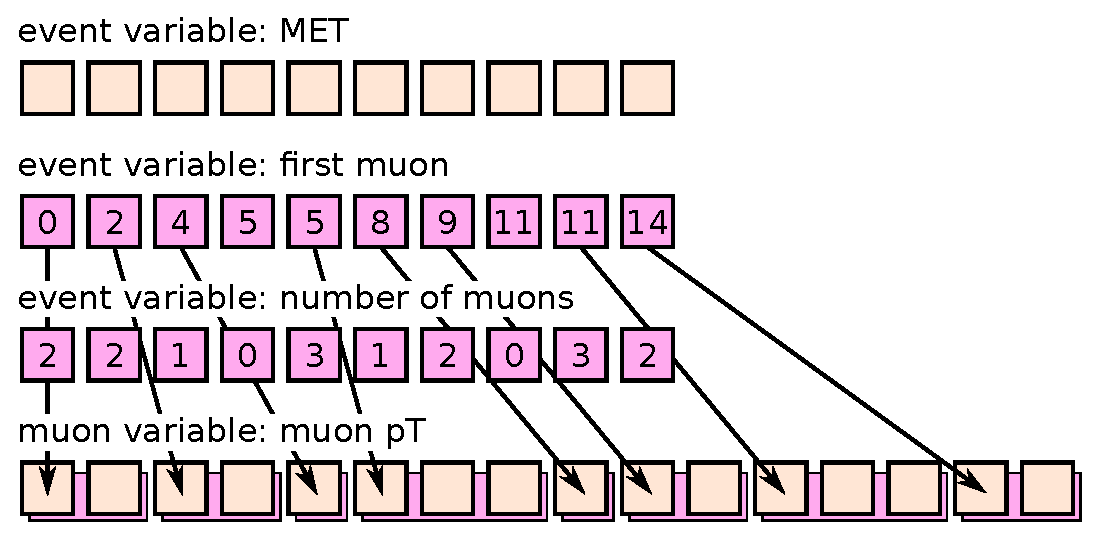
\includegraphics[width=0.8\linewidth]{hierarchical_arrays.pdf}

\item Parquet uses logical type systems to provide Avro objects.

\item ROOT's physical types are streamers, logical types are C++.
\end{itemize}
\end{frame}

\begin{frame}{Why use alternate formats?}
\vspace{0.25 cm}
\begin{block}{Transient: getting data into another system}
\begin{itemize}
\item Necessary in many cases: the C++/Java barrier is particularly difficult to overcome.
\end{itemize}
\end{block}

\begin{block}{End-stage of analysis in another system}
\begin{itemize}
\item If we're making ntuples anyway, the format should be chosen with the analysis tool in mind: ROOT or otherwise.
\end{itemize}
\end{block}

\begin{block}{Releasing open data to the public}
\begin{itemize}
\item Current format probably inhibits use. Avro/Parquet on popular analysis clouds (AWS, Google Cloud, Azure, etc.)?
\end{itemize}
\end{block}

\begin{block}{New primary data storage format?}
\begin{itemize}
\item Would require {\it considerable} thought.
\end{itemize}
\end{block}
\end{frame}

\begin{frame}{Today's talks}
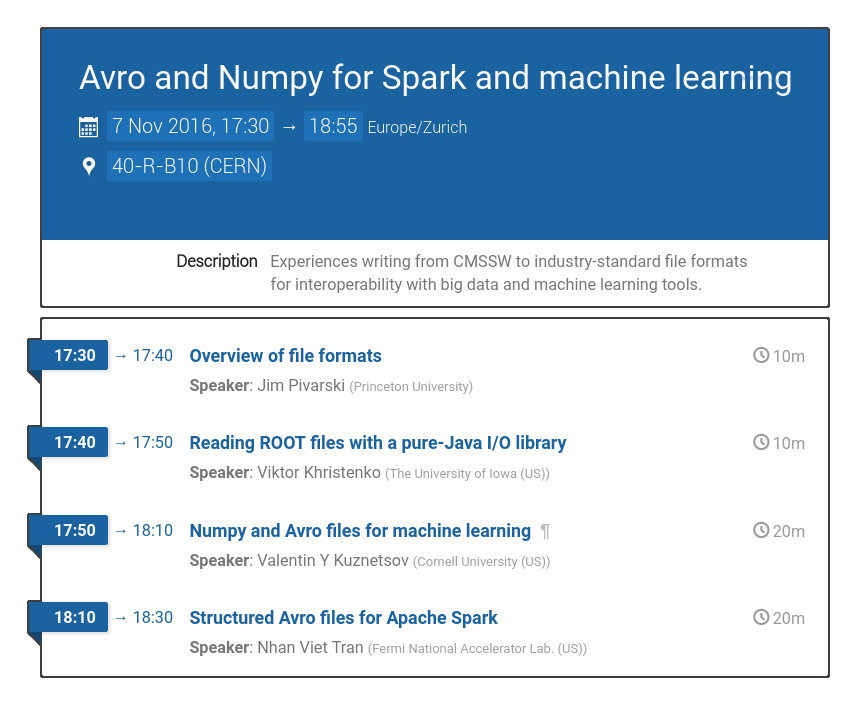
\includegraphics[width=\linewidth]{schedule.png}
\end{frame}

\end{document}
